% =====================================================================
%  Air void fraction (% of reference) -- 3 stacked bar panels
%  Panel 1: 8 mm solid step      (Experiment vs 2D Simulation)
%  Panel 2: B3 bars              (Experiment vs 2D Simulation)
%  Panel 3: B3 bars original vs shifted (Exp vs 2D Sim vs 2D Sim shifted)
%
%  Percentages are precomputed to match the Python pct() logic:
%    - script 1: values <= 0.5 % are clamped to a 2 % stub (EPS_PCT=2)
%      -> affects only STEP/sim/case6 (true 0.4375 % -> drawn as 2 %)
%
%  This is a standalone minimal working example. To drop it into your
%  document, copy everything between \begin{tikzpicture}...\end{tikzpicture}
%  (and the \definecolor lines + \pgfplotsset block into your preamble).
% =====================================================================
\documentclass[tikz,border=2pt]{standalone}
\usepackage{pgfplots}
\usepackage{amsmath}
\pgfplotsset{compat=1.18}
\usepgfplotslibrary{groupplots}

% ---- Colours (match matplotlib: grey, orange, forestgreen) ----------
\definecolor{expgrey}{HTML}{7F7F7F}
\definecolor{simorange}{HTML}{FF7F0E}
% \definecolor{simgreen}{HTML}{228B22}

% ---- Shared style: edit these to fine-tune all panels at once -------
\pgfplotsset{
  voidbar/.style={
    width=7.5cm, height=3.5cm,
    ybar=2pt,                 % gap between bars within a case-cluster
    bar width=10pt,           % bar thickness
    xmin=0.5, xmax=4.5,
    xtick={1,2,3,4},
    xticklabels={Case 3, Case 4, Case 5, Case 6},
    ymin=0,
    ymajorgrids=true,
    grid style={line width=0.6pt, color=black!18},
    tick align=outside,
    tick label style={font=\small},
    ylabel={Relative \\accumulation\\ size [\%]},
    ylabel style={font=\small, align=center},
    title style={font=\normalfont, at={(-0.35,0.9)}, anchor=south west},
    % uniform little filled squares for the legend
    legend image code/.code={\draw[#1] (0cm,-0.09cm) rectangle (0.28cm,0.16cm);},
    legend cell align=left,
  }
}

\begin{document}
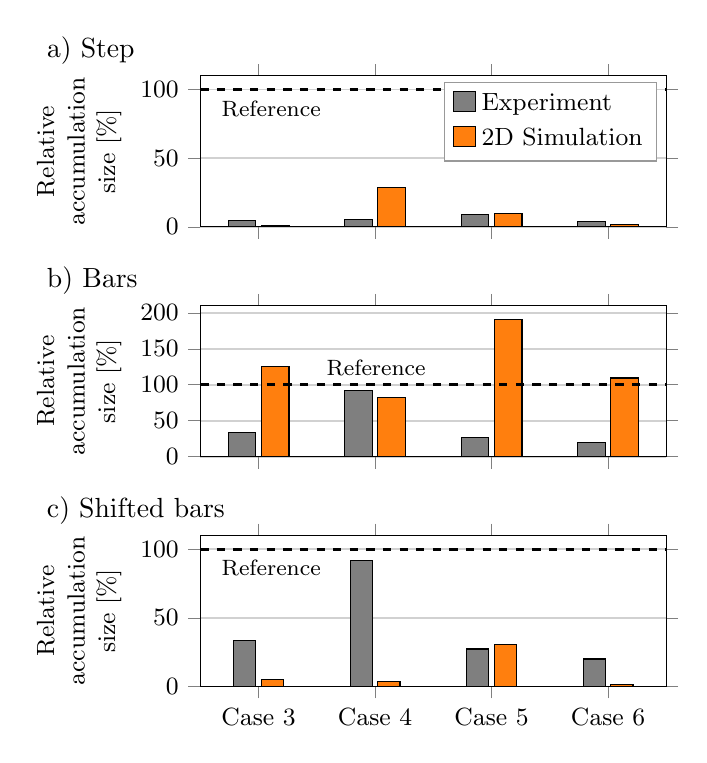
\begin{tikzpicture}
\begin{groupplot}[
  voidbar,
  group style={
    group size=1 by 3,
    vertical sep=1.0cm,
    % only the bottom panel shows the case labels (toggle if you want all)
    xticklabels at=edge bottom,
  },
]

% ---------------- Panel 1 : Step ----------------
\nextgroupplot[
  title={a) Step},
  ymax=110,
  legend style={at={(0.98,0.96)}, anchor=north east, font=\small,
                fill=white, draw=black!40, row sep=1pt},
]
\addplot[fill=expgrey,  draw=black] coordinates {(1,4.7619)(2,5.7143)(3,9.0909)(4,4.0)};
\addlegendentry{Experiment}
\addplot[fill=simorange,draw=black] coordinates {(1,0.9012)(2,28.6552)(3,9.4737)(4,2.0)};
\addlegendentry{2D Simulation}

% 100 % reference line
\draw[black, dashed, line width=1pt] (axis cs:0.5,100) -- (axis cs:4.5,100);
\node[anchor=north west, font=\footnotesize] at (axis cs:0.6,99) {Reference};

% ---------------- Panel 2 : Bars ----------------
\nextgroupplot[
  title={b) Bars},
  ymax=210,                 % matches matplotlib auto-scale (max*1.15)
]
\addplot[fill=expgrey,  draw=black] coordinates {(1,33.3333)(2,91.4286)(3,27.2727)(4,20.0)};
\addplot[fill=simorange,draw=black] coordinates {(1,125.3033)(2,82.7586)(3,190.1316)(4,109.375)};
\draw[black, dashed, line width=1pt] (axis cs:0.5,100) -- (axis cs:4.5,100);
\node[anchor=south west, font=\footnotesize] at (axis cs:1.5,99) {Reference};

% ---------------- Panel 3 : Shifted bars ----------------
\nextgroupplot[
  title={c) Shifted bars},
  ymax=110,
  bar width=8pt,            % slightly thinner: 3 bars per case
]
\addplot[fill=expgrey,  draw=black] coordinates {(1,33.3333)(2,91.4286)(3,27.2727)(4,20.0)};
% \addplot[fill=simorange,draw=black] coordinates {(1,125.3033)(2,82.7586)(3,190.1316)(4,109.375)};
\addplot[fill=simorange, draw=black] coordinates {(1,4.974)(2,3.8966)(3,30.5921)(4,1.5625)};
\draw[black, dashed, line width=1pt] (axis cs:0.5,100) -- (axis cs:4.5,100);
\node[anchor=north west, font=\footnotesize] at (axis cs:0.6,99) {Reference};

\end{groupplot}
\end{tikzpicture}
\end{document}